\documentclass[12pt]{article}
\usepackage[utf8]{inputenc}
\usepackage[T1]{fontenc}
\usepackage{lmodern}  % for better quality fonts
\usepackage{amsmath,amssymb}
\usepackage{fontawesome}
\usepackage{lipsum}
\usepackage{hyperref}
\usepackage[margin=3em, top=0.5em]{geometry}
\usepackage{multirow}
\usepackage{array} % For extended tabular features
\usepackage{graphicx} % For better vertical alignment
\usepackage{xcolor}
\usepackage[explicit]{titlesec}
\usepackage{tikz}
\usepackage{enumitem}

%custom color definitions
\definecolor{navy}{HTML}{1c398d}
\definecolor{softblack}{HTML}{333333}
\definecolor{subtextgray}{HTML}{768699}
\definecolor{LinkedinBlue}{HTML}{0a66c2}

%tabular column aligners & settings
\newcolumntype{L}[1]{>{\raggedright\arraybackslash}p{#1}}
\newcolumntype{R}[1]{>{\raggedleft\arraybackslash}p{#1}}
\setlength{\tabcolsep}{1.6em}

%label item settings -> small dot & pos
\renewcommand{\labelitemi}{\raisebox{0.1em}{$\cdot$}}

%title settings
\titlespacing{\section}{0em}{-1em}{0.1em}
\newcommand{\raisedrulefill}[2][0ex]{\leaders\hbox{\rule[#1]{1pt}{#2}}\hfill}
\titleformat{\section}{\normalfont\scshape\large\color{softblack}}{}{0pt}{\textcolor{softblack}{#1\,\raisedrulefill[0.25em]{0.2pt}}} 

\begin{document}

\begin{center}
  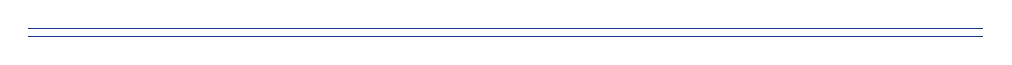
\begin{tikzpicture}
    \draw[thin, navy] (0,0) -- (\linewidth, 0);
    \draw[thin, navy] (0,-0.1) -- (\linewidth,-0.1);
  \end{tikzpicture}

  \vspace{0.4em}
  
  \begin{tabular}{@{} L{0.3\textwidth} c R{0.3\textwidth} @{}}
    \faEnvelope \hspace{0.1em} \color{softblack} \href{mailto:me@leosharif.com}{me@leosharif.com} & \color{softblack} \multirow{2}{*}{\huge\scshape Leo Sharif} & \faGithub \hspace{0.1em} \color{softblack} \href{https://github.com/Realaiz}{Leo Sharif} \\
    \faPhone \hspace{0.1em} \color{softblack} +61 420-677-719 & & \textcolor{LinkedinBlue} \faLinkedinSquare \hspace{0.1em} \color{softblack} \href{https://www.linkedin.com/in/leo-sharif-1a6866193/}{Leo Sharif} \\
    & \color{softblack} \normalsize \color{subtextgray} Mathematics \& Finance & \faHome \hspace{0.1em} \color{softblack} \href{https://leosharif.com}{leosharif.com} \\
  \end{tabular}

  \vspace{0.4em}

  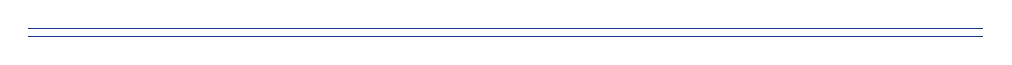
\begin{tikzpicture}
    \draw[thin, navy] (0,0) -- (\linewidth,0);
    \draw[thin, navy] (0,-0.1) -- (\linewidth,-0.1);
  \end{tikzpicture}
\end{center}


% Education Section
\section{education}
\textbf{Bond University} \hfill {Gold Coast, QLD} \\
\indent \textit{\color{subtextgray}B. Actuarial Science, Major in Finance} \hfill \textit{\color{subtextgray}Feb 2022 - May 2024}
\begin{itemize}[noitemsep, topsep=0em, left=0.8em]
  \item 75\% Major WAM, Investment Group, Actuarial Society, Actuaries Institute Completion: CS, CM, CB
  \item Coursework: Mathematical Statistics, Stochastic Processes, Econometrics, Finance Mathematics, Portfolio Analysis, Survival Analysis, Risk Management, Financial Models, Game Theory, Survival Analysis
\end{itemize}

\textbf{Academy of Interactive Technology} \\
\indent \textit{\color{subtextgray}Diploma of Full Stack Development}
\begin{itemize}[topsep=0em, left=0.8em]	
  \item 78\% WAM, Developed a password manager and a real estate portfolio management tool, showcasing strong problem-solving skills and industry-standard security practices.
\end{itemize}

\vspace{1em}

\section{work \& experience}

\vspace{0.20em}

\textbf{Nabla} \hfill {Gold Coast, QLD} \\
\indent \textit{\color{subtextgray}President}
\begin{itemize}[noitemsep, topsep=0em, left=0.8em]
  \item Founded the Quantitative Finance Society in response to a growing demand for quantitative skills in investment analysis; successfully onboarded an initial team of dedicated and talented members to drive the society's objectives and promote a strong foundation for future growth.
  \item	Initiated the development of a heat map for option strike prices, utilising Python and C++ to create an interactive, visually engaging dashboard that simplifies complex financial data for members.
  \item Tested the hypothesis that trading based on technical indicators lacks merit by employing machine learning to automate the analysis of these indicators, aiming to determine their effectiveness in generating alpha.
\end{itemize}

\textbf{Sitesec} \hfill {Gold Coast, QLD} \\
\indent \textit{\color{subtextgray}Systems Engineer}
\begin{itemize}[noitemsep, topsep=0em, left=0.8em]
  \item Managed databases and ensured data integrity, accuracy, and availability for various stakeholders, including project managers, clients, and regulatory bodies.
  \item	Leveraged data analytical techniques to map and plan construction projects, optimising resource allocation and project timelines.
  \item Streamlined physical workflow by delegating tasks and managing projects effectively, resulting in increased efficiency and productivity.
  \item Improved technical workflow by implementing firmware upgrades and enhancing system performance and security.
\end{itemize}



\textbf{Eante} \hfill {Brisbane, QLD} \\
\indent \textit{\color{subtextgray}Software Development Intern}
\begin{itemize}[noitemsep, topsep=0em, left=0.8em]
  \item Implemented a micro interest-earning system with visual representations to encourage long-term saving habits.
  \item	Shadowed experienced developers working on explosion mapping software for a mining company project, gaining exposure to diverse industries and improving adaptability and problem-solving skills in various contexts.
  \item Enhanced communication and teamwork abilities through active collaboration with software development team.
\end{itemize}

\vspace{0.20em}

\section{Quantitative Research Projects}

\section{Skills}

\section{Additional Info}



\end{document}



